\documentclass[10pt,a4paper]{article}
\usepackage[utf8]{inputenc}
\usepackage{amsmath}
\usepackage{amsfonts}
\usepackage{amssymb}
\usepackage{graphicx}
\usepackage{subcaption}

\begin{document}


\begin{figure}[!h]
	\centering     %%% not \center

	\subfigure[Passo 1]{\label{fig:a}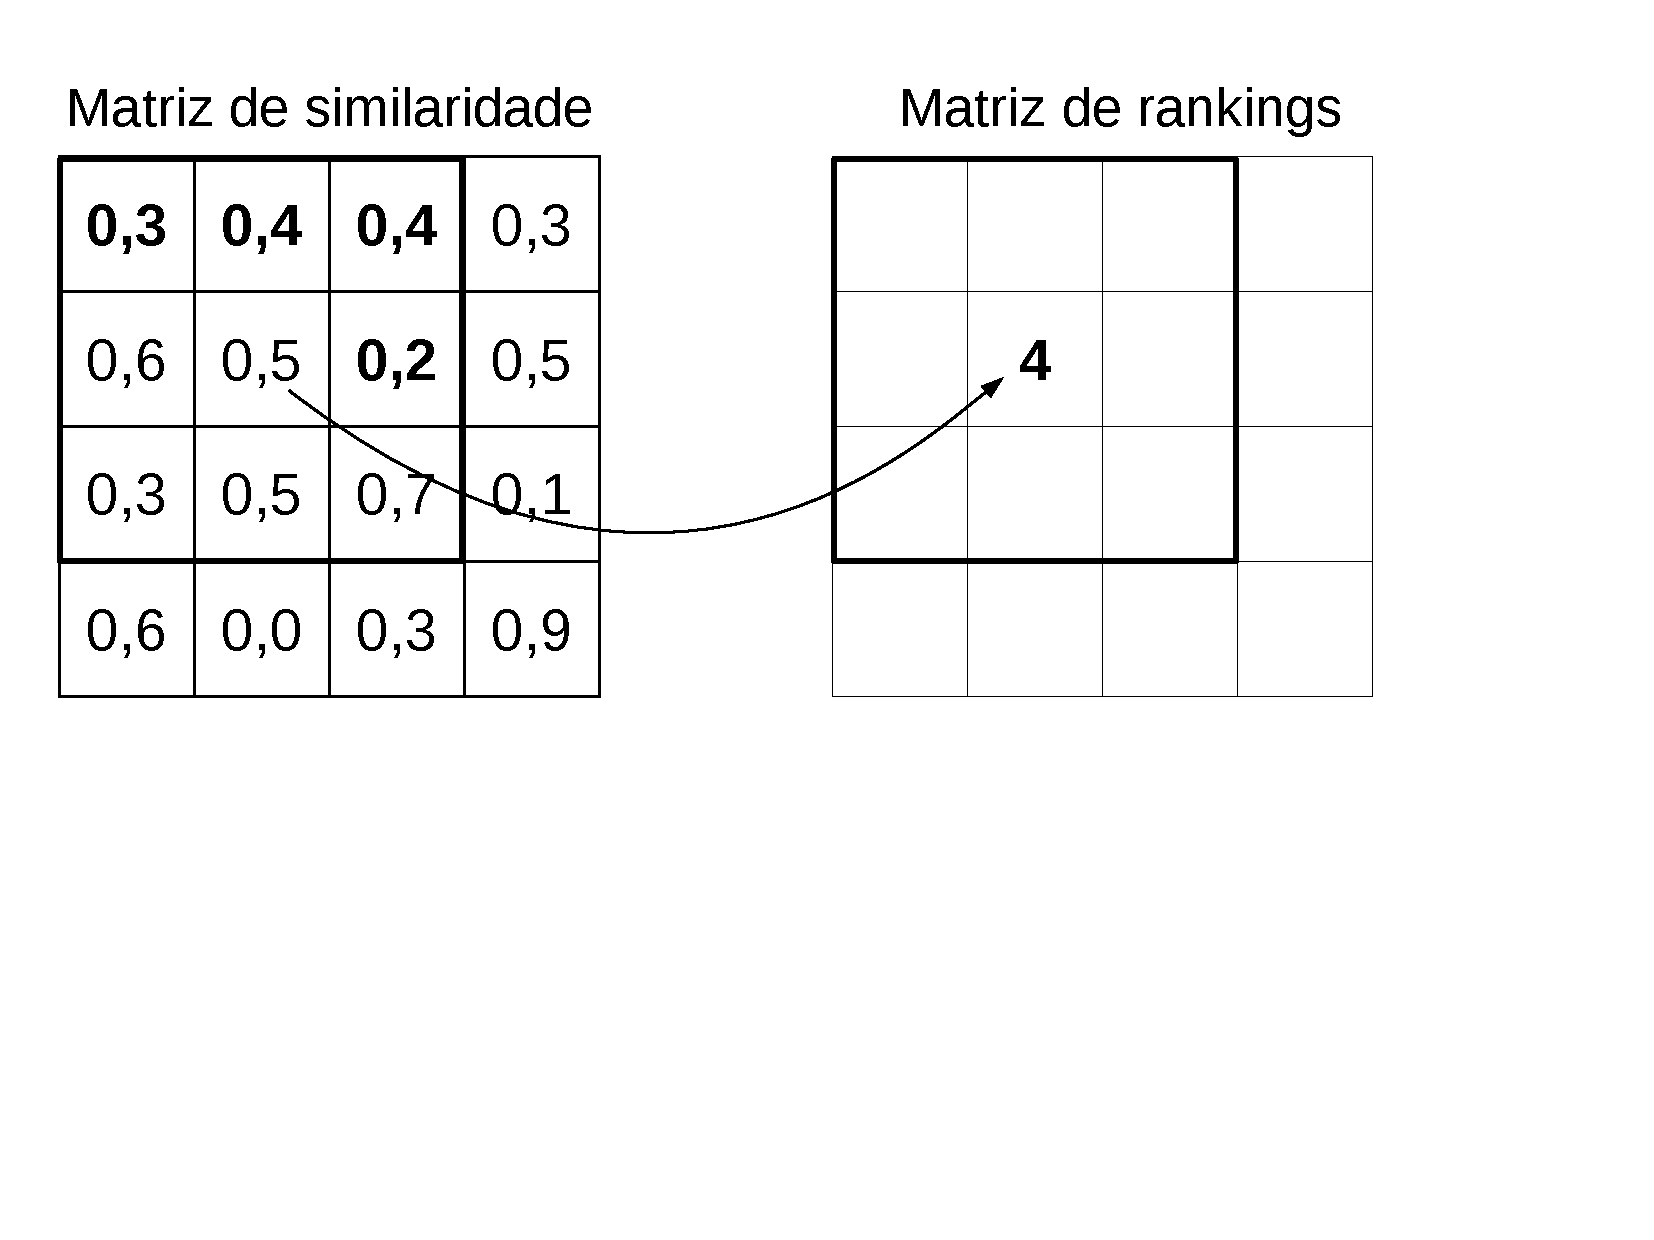
\includegraphics[width=60mm]{c99-matrizes.pdf}
	\subfigure[Passo 2]{\label{fig:b}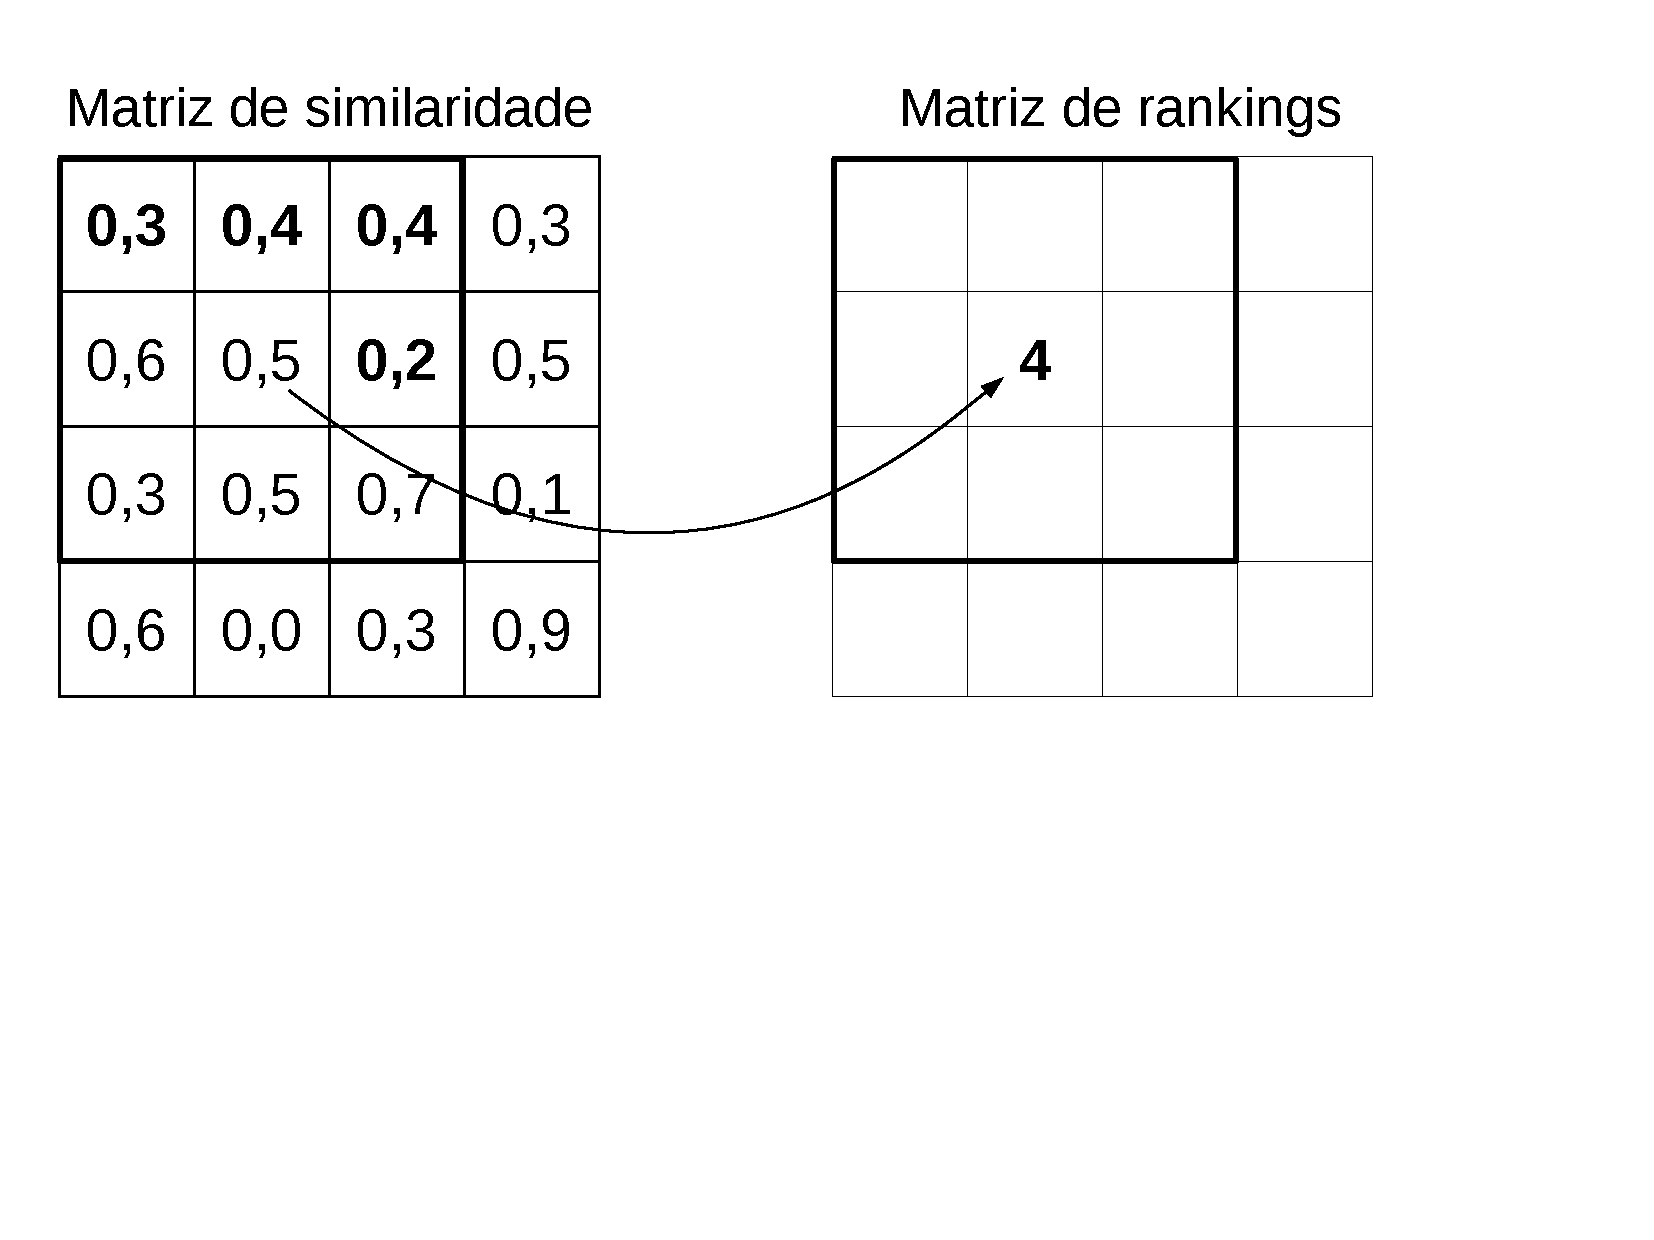
\includegraphics[width=60mm]{c99-matrizes.pdf}
	
	\caption{Exemplo de construção de uma matriz de rankings.%~\cite{Choi2000}.
	}
	\label{fig:exemplomatrixrank}
\end{figure}



\begin{figure}[h!]
\center
	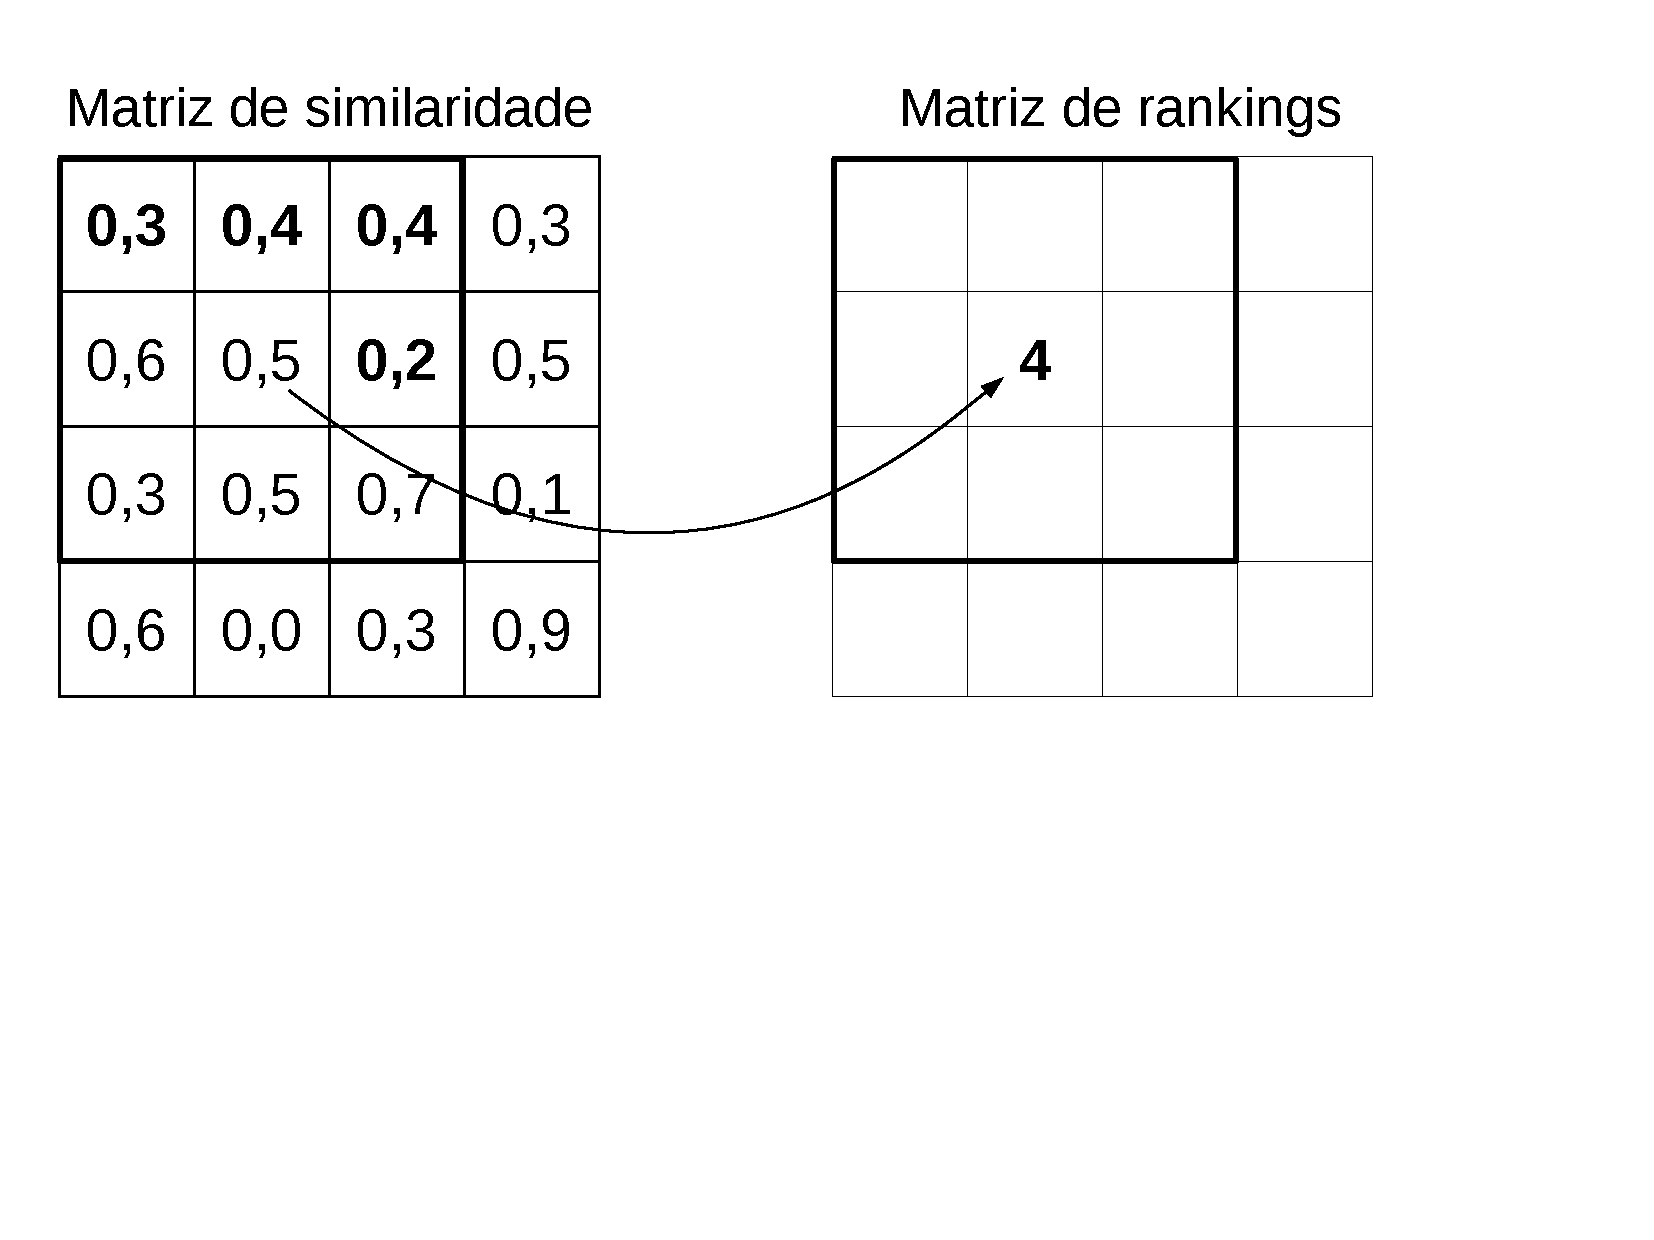
\includegraphics[trim={ 0 60 0 66 },clip,page=1,width=0.8\textwidth]{c99-matrizes.pdf}

	\caption{Processo de deslocamento da janela deslizante. Os quadrados numerados representam as sentenças e os retângulos representam os blocos de texto a serem comparados. O deslocamento movimenta o candidato a limite e por consequência os blocos que o antecede e sucede.}
	\label{fig:TT-slidingwindow}
\end{figure}


\end{document}